\section{Soma dos Subconjuntos}

\subsection{Enunciado}

Assim como definido no enunciado do Trabalho 3 da disciplina, o problema é o seguinte:

\textsc{Subset-Sum}: dado um conjunto finito de números naturais $S$ e um valor $t \in \mathbb{N}$, existe algum subconjunto não-vazio $S' \subseteq S$ em que seus elementos somados resultem em $t$?

Ou pode-se definir o problema mais formalmente como uma linguagem:

\textsc{Subset-Sum} $= \{ \langle S, t \rangle$ : existe um subconjunto $S' \subseteq S$ tal que $t = \sum_{s \in S'}s \}$.

Trata-se de um \textbf{problema de decisão}, uma vez que é esperada uma resposta \textit{sim} ou \textit{não}.

\subsection{Explicação}

Pensando em uma linguagem de programação, pode-se imaginar o conjunto $S$ como um vetor de dados \texttt{unsigned int} de tamanho \texttt{n}, e procura-se por algum subconjunto dele em que a soma dos valores resulte em um valor de entrada \texttt{t}.

\begin{figure}[h]
	\centering
	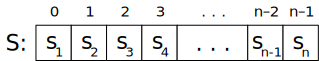
\includegraphics[scale=0.9]{./input/vetor.pdf}
	\caption{Ilustração de um vetor para o conjunto $S$. \label{fig:vetor}}
\end{figure}

Pode-se observar que há uma grande quantidade de subconjuntos para o vetor \texttt{S} em função do seu tamanho \texttt{n}, pois o total de subconjuntos é:

$$
	\sum_{i=1}^{n} {n \choose i} = {n \choose 1} + {n \choose 2} + \cdots + {n \choose n-1} + {n \choose n} = 2^n - 1
$$

Ou seja, é o número de subconjuntos com 1 elemento, mais o número de subconjuntos com 2 elementos etc, até o último subconjunto que é quando $S' = S$, e desconsiderando o conjunto vazio quando $i = 0$.

Dado esse total de subconjuntos possíveis, no pior caso, para encontrar um subconjunto que satisfaça o \textsc{Subset-Sum} e responda \textit{sim}, um algoritmo ingênuo teria complexidade exponencial de $O(2^n)$, pois verificaria todos eles. Por exemplo, um conjunto $S$ de tamanho $n = 100$ tem $2^{100} - 1 = 1\ 267\ 650\ 600\ 228\ 229\ 401\ 496\ 703\ 205\ 375$ subconjuntos não-vazios.

